\documentclass[a4paper, 12pt]{article}
\usepackage[french]{babel}
\usepackage[T1]{fontenc}
\usepackage[utf8]{inputenc}
\usepackage[left=2cm,right=2cm,top=3cm,bottom=2cm]{geometry}
\usepackage{graphicx}
\usepackage{xcolor}
\usepackage{color}
\usepackage{ulem}
\usepackage{setspace}
\usepackage{fancyhdr}
\usepackage{float} 
\usepackage[section,above,below]{placeins}
\usepackage[final]{pdfpages}

 
\usepackage{tcolorbox,listings}
\usepackage{fullpage}
\usepackage{color}
 \usepackage[backend=bibtex]{biblatex}
\definecolor{darkWhite}{rgb}{0.94,0.94,0.94}
 
\lstset{
    backgroundcolor=\color{darkWhite},
    breakatwhitespace=false,
    breaklines=true,
    captionpos=b,
    commentstyle=\color{red},
    deletekeywords={...},
    escapeinside={\%*}{*)},
    extendedchars=true,
    keepspaces=true,
    keywordstyle=\color{blue},
    language=C,
    morekeywords={*,...},
    showspaces=false,
    showstringspaces=false,
    showtabs=false,
    stepnumber=1,
    stringstyle=\color{red},
    tabsize=4,
    title=\lstname,
    numbers=left, numberstyle=\tiny, stepnumber=1, numbersep=5pt,
}
 
\lstdefinestyle{frameStyle}{
    basicstyle=\footnotesize,
    numbers=left,
    numbersep=2pt,
    numberstyle=\tiny\color{black}
}
 
\tcbuselibrary{listings,skins,breakable}
 
\newtcblisting{customFrame}{
    arc=0mm,
    top=0mm,
    bottom=0mm,
    left=3mm,
    right=0mm,
    width=\textwidth,
    listing only,
    listing options={style=frameStyle},
    breakable
}

\renewcommand{\contentsname}{Sommaire}

\usepackage{footnote}

\begin{document}

\begin{titlepage}
	\centering
	
\includegraphics[width=1\textwidth]{univ.jpg}\par\vspace{1cm}
	{\scshape\LARGE PROJET DE FIN D'ÉTUDES\par}
	\vspace{1cm}
	{\scshape\Large\bfseries EVERNET - TRANMISSION DE SLOTS ET NETWORK CODING
 \par}
 	\vspace{0.5cm}
 {\Large\bfseries Sujet proposé par Serge CHAUMETTE \par}
 
 	
	\vspace{1.5cm}
	{\huge\bfseries CAHIER DES CHARGES  \par}
	\vspace{1cm}
	
	
	{\Large\itshape\bfseries BALLION Lucas  \par}
	{\Large\itshape\bfseries DIALLO Abdoul   \par}
	{\Large\itshape\bfseries DIALLO Thierno   \par}
	{\Large\itshape\bfseries HOARAU Raphael   \par}
	{\Large\itshape\bfseries PORTEJOIE Sarah  \par}
	{\Large\itshape\bfseries KARA Zoubir  \par}
		

	\vspace{1cm}
	
	
	{\Large\bfseries Master 2 Informatique   \par}
	\vspace{0.5cm}
	{\Large\bfseries Chargés de TD : \\
	Pascal DESBARATS	   \par}
	\vspace{1.5cm}

	
	
% Bottom of the page
	{\large\bfseries \today\par}
\end{titlepage}

\tableofcontents
\newpage
\section{Introduction}

Dans le cadre de notre Cursus de Master 2 en Informatique à l'Université de Bordeaux, nous allons présenter dans ce cahier des charges notre projet de fin d'études Evernet réalisé par groupes de six étudiants. Nous travaillons avec Monsieur \textbf{Serge CHAUMETTE} notre client et monsieur \textbf{Pascal DESBARATS} chargé de l'encadrement de nos travaux dirigés.\\

L'objectif de ce projet est de permettre la transmission efficace d'images en toute confidentialité entre téléphones mobiles dans un environnement non sécurisé, sans connexion Internet, et ce, en utilisant le service de messagerie SMS tout en répartissant sur l'ensemble des participants le coût énergétique et l'empreinte CO2. 

Les téléphones des utilisateurs serviront de relais entre l'émetteur et le destinataire de l'image. Pour cela, l'image sera découpée en paquets de petite taille que l'on nommera slots, qui seront envoyés vers les mobiles d'autres participants choisis au hasard, ces derniers les retransmettront à leur tour dans des délais raisonnables.
Les numéros de mobiles des participants doivent rester confidentiels. Afin de garantir l'anonymat, un serveur central sera donc utilisé pour gérer l'association pseudonyme-numéro de téléphone.

Ce projet a été découpé en trois parties : 
\begin{enumerate} 
    \item le serveur central et PKI
    \item la transmission des slots et le Network Coding
    \item le système de visualisation et de débug
\end{enumerate}

Notre mission dans de ce projet consiste à étudier et à mettre en place le système de transmission des slots en utilisant le Network Coding. Pour ce faire, nous devons découper l'image à envoyer en plusieurs paquets, assurer leur acheminement en toute sécurité dans le réseau, tout en veillant à l'équilibre de la charge énergétique et de l'empreinte carbone.
Nous présenterons ainsi dans ce cahier des charges les différentes contraintes et prévisions, ainsi que les besoins associés au projet. 
%pour brouiller les pistes des observateurs extérieurs.


\section{Analyse de l'existant}

Plusieurs applications pour téléphone mobile, permettant l'envoi de messages et/ou d'images, sont déjà disponibles sur le marché. Parmi celles-ci, on retrouve notamment WhatsApp, Telegram et Signal.
\begin{itemize}
    \item WhatsApp permet l'envoi de messages et d'images en utilisant une connexion internet fixe ou par un réseau internet mobile (3G,4G). Elle offre un chiffrage de bout en bout des communications et compte plus de 2 milliards d'utilisateurs à travers le monde. En 2014, l'application est rachetée par Facebook. Bien que les communications soient chiffrées, WhatsApp fait face à des critiques concernant la confidentialité des données personnelles échangées sur la plateforme, notamment depuis son rachat en 2014 et la mise en place de nouvelles conditions d'utilisations début 2021, qu'il est obligatoire d'accepter afin de continuer à utiliser le service. Ceci a eu pour conséquence, une fuite d'un certain nombre d'utilisateurs vers des services concurrents.
    \item Telegram est une application de messagerie permettant d'échanger des messages et des documents de manière sécurisée. La partie cliente est libre alors que la partie serveur est propriétaire. A l'origine, l'application a été développée par deux frères russes Nikolaï et Pavel Dourov afin de pouvoir communiquer tout en évitant la censure. Certains experts en sécurité émettent des doutes sur le mode d'authentification de Telegram en expliquant qu'il serait possible d'usurper l'identité d'un utilisateur en interceptant le code SMS de vérification. Actuellement l'application compte plus de 500 millions d'utilisateurs à travers le monde.
    \item Signal est une application conçue dans le but d'être la plus sécurisée possible, de plus, elle réalise une collecte minime des données personnelles des utilisateurs. Elle est distribuée sous licence libre. Elle est financée par la Signal Foundation qui est une association à but non lucratif. Son haut niveau de sécurité fait qu'elle est recommandée par des personnalités comme Edward Snowden ou Elon Musk. La commission européenne recommande à son personnel l'utilisation de Signal. Moins utilisée que ses concurrents, signal connaît un certain succès, notamment depuis le changement des conditions d'utilisation de WhatsApp, ce qui entraîne 47 millions de téléchargements en deux semaines pour Signal.
\end{itemize}
L'application Evernet offre un protocole d'échange d'image sécurisé. Ses principales différences vis à vis des solutions actuelles existantes est le fait qu'elle n'utilise que les SMS pour échanger les données. L'autre particularité d'Evernet contrairement aux autres solutions disponibles, est qu'elle permet uniquement l'échange d'image et non de messages et autres types de documents.

Le network coding est un thème de recherche qui a été récurant à la fin des années 90 et au début des années 2000. Son objectif est d'améliorer le débit, l'efficacité et l'évolutivité d'un réseau de communication. Un autre avantage du network coding est qu'il permet d'augmenter la résistance du réseau aux attaques. Son principe de base consiste à faire transiter sur un lien de communication plus d'un paquet à la fois. Lorsqu'un noeud du réseau reçoit deux paquets celui-ci va agréger les deux paquet de manière à ne faire circuler sur le lien qu'un seul paquet. Pour parvenir à cela, une opération binaire (par exemple un xor) va être faite sur le payload des deux paquets pour ne constituer qu'un seul paquet. On peut donc faire transiter sur un seul lien plus de données dans la même unité de temps et on accroît donc le débit du réseau, de plus, le codage appliqué au payload va permettre de renforcer la sécurité globale du réseau. L'utilisation de ce protocole dans notre projet va permettre d'améliorer les performances globales du réseau ainsi que sa sécurité.    

\section{Analyse des besoins}
    \subsection{Besoins fonctionnels}
        
        
        
        \subsubsection{Ajouter un contact}
        
         Pour ajouter un contact dans la liste de contacts, l'utilisateur doit cliquer sur un bouton "Ajouter un contact" qui ensuite le redirige vers une page lui demandant de   saisir le pseudonyme du contact correspondant.
         Si ce pseudonyme est valide alors la demande est envoyée. Lorsqu'elle est acceptée, chacun des deux utilisateurs  ajoute l'autre dans sa liste de contacts.
        \subsubsection{Ajouter un nouveau groupe (optionnel)}
        Un utilisateur peut créer un groupe de discussions dans lequel il peut ajouter d'autres personnes en utilisant la même technique que celle de la section "Ajouter un contact".\\
        Le créateur du groupe en devient l'administrateur.Il aura donc le pouvoir d'ajouter ou de retirer des personnes, de supprimer des messages qu'il jugera contraire à l'étique du groupe et même de fermer le groupe.\\
        Un groupe fermé ne peut plus être récupéré et le nombre maximum de personnes autorisé par groupe est de 100.

        \subsubsection{Sélection de destinataire}
        Dans un menu contenant la liste des contacts, l'utilisateur devra choisir le destinataire depuis cette liste en clinquant sur le pseudonyme correspondant au destinataire.\\
        Pour rappel, un contact peut être une personne ou un groupe de personnes.\\
        
        
        \subsubsection{Sélection de l'image à envoyer}
        L'image à envoyer doit être sélectionnée depuis la galerie de photos du téléphone de l'utilisateur.
         L'application doit prendre en charge trois types de formats d’images qui sont : jpg, jpeg et png. 
        \subsubsection{Envoi de l'image}
        
        Une fois l'image sélectionnée, l'utilisateur appuie sur un bouton "envoyer" afin de déclencher l'envoi.\\
        Cet envoi contient plusieurs étapes, qui sont:\\
            \begin{itemize}
              \item \textbf{Encodage de l'image dans un format supportable par le mode SMS (sans internet)}\\
              On pourra par exemple choisir de les encoder en binaire ou en décimal. Ces deux formats sont plutôt simple à implémenter dans le langage de programmation choisi dans ce projet
              \item \textbf{Découpage de l'image encodée en des slots de même taille} \\
              Le nombre de slots dépendra de la taille en octet qu'on peut envoyer d'un seul coup, du nombre de numéros intermédiaires que le serveur nous aura renvoyer. 
              L'en-tête du message à envoyer ne contient pas que du slot de l'image,il contient également
              la position du slot pour la reconstruction par le destinataire,du nombre total de slots que contiendra l'image et d'une durée de vie (ttl time to live en Anglais).
              Avant l'envoi il faudra chiffrer le slot par la clé publique du destinataire ou expéditeur.\\
              Le choix définitif de la clé à utiliser revient au développeur .Il faudra toute fois qu'il  indique dans le rapport final son choix et ses motivations. 
              \item \textbf {Fin de l'envoi} \\
              À la fin de l'envoi, une boîte de dialogue informe l’utilisateur que son image est bien envoyée.  

            \end{itemize} 
        \subsubsection{Réception des slots de l'image par le destinataire}
        Lorsqu'un destinataire reçoit un paquet contenant un slot,il le déchiffre grâce aux clés,place le slot à sa position et regarde ensuite s'il reste d'autres paquets.
        si oui, il attend. Sinon il affiche l'image reçue.
        \subsubsection{Gestions des paquets par les noeuds intermédiaires}
        Un noeud intermédiaire qui reçoit un paquet doit le gérer de la façon suivante:\\
        \begin{itemize}%% Ajouter ici le cas d'utilisation du network coding
            \item Si le ttl est égal à 0, alors il y'a 2 cas :\\
            Soit on jette le paquet, soit on l'envoie directement à la destination.
            Libre choix au développeur d'implémenter soit un, soit les deux cas. 
            \item Si le ttl est diffèrent de 0, il fait une requête au serveur pour qu'il lui renvoie d'autres numéros intermédiaires puis renvoie le paquet à ces destinations.
        \end{itemize}
        
                
            
            
            
        \subsubsection{Gestion de l'équilibre carbone}
            La gestion de l'équilibre carbone est l'un des points clef de cette application. Il est nécessaire d'avoir une distribution efficace du trafic sur le réseaux afin de répartir équitablement la charge sur les noeuds du réseau (les téléphones dans ce cas ci).\\
            De plus l'utilisation d'un \textbf{Network Coding} efficace rendra le réseaux résilient, rendant possible la correction d'erreur. Correction qui diminuera ainsi le nombre de paquet sur le réseaux en évitant les retransmissions des données perdues/erronées.
        
        
    \subsection{Besoins non fonctionnels}
        
        \subsubsection{Portabilité sur les différentes versions d'Android}
            L'application qui doit être développée doit être compatible avec un maximum de terminaux android. Il est donc important de choisir une version minimale requise d'android permettant la plus large compatibilité possible. Il apparaît que rendre l'application compatible avec les systèmes android 4.4 et ses version ultérieure, permet à environ 98\%
            des terminaux android, d'être compatible avec notre application ce qui est nettement suffisant. Notre application sera donc compatible avec les systèmes android 4.4 et ultérieur.
        
        \subsubsection{Langage de programmation}
            L'application doit être conçue pour fonctionner sous le système d'exploitation mobile android. Ce qui nécessite d'utiliser un environnement de développement approprié.
            Il a donc été choisi d'utiliser Android Studio. Java est le langage de programmation qui a été retenu pour ce projet . Ce dernier est disponible sur Android Studio et est connu par tous les membres de notre groupe.
        
        \subsubsection{Compatibilité avec les autres parties du projet global}
            Le projet Evernet étant divisé en trois sous-projets, notre application doit être en mesure de s'intégrer avec les deux autres sous-projets afin que le projet global puisse être fonctionnel. Elle devra donc être en capacité d'utiliser les services de sécurité offerts par le serveur fourni par le groupe 1. Le groupe 3 devant retracer le parcours des paquets sur le réseau, notre entête devra donc contenir suffisamment d'informations afin que ceci soit possible. Des informations comme la source initiale, la destination finale seront indispensables au groupe 3 et devront être présentes dans l'entête.  
        
        \subsubsection{Simplicité d'utilisation}
            
            La simplicité d'utilisation est essentiel pour l'expérience utilisateur. Une interface simple et ergonomique est nécessaire au bon développement de l'application. Une interface trop complexe conduira à une non-utilisation de l'application par les utilisateurs qui se tourneront vers des solutions plus simples.
            Pour ce faire un respect des règles d'Interface Homme-Machine est nécessaire. Ces règles posent un cadre qui permet au développeur de réaliser une interface la plus ergonomique et simple possible. Ainsi l'application est plus agréable et simple à utiliser.

\section{Contraintes}
Ce projet amène différentes contraintes techniques qui sont :
\\

\begin{itemize}
\item [•]{Application du Network coding}
            
            La pierre angulaire de ce projet est l'utilisation du \textbf{Network Coding}. Cette façon de gérer les paquets SMS circulant sur le réseaux permet d'optimiser le trafic, et d'augmenter la sécurité.
            Lorsque plusieurs paquets ayant la même destination arrivent sur un noeud du réseau, les données que ces paquets portent sont combinées pour former une seule donnée. On peut ainsi envoyer un seul paquet contenant les données combinées et la façon dont les données sont combinées.
            On réduit ainsi le nombre de paquet nécessaire pour transmettre l'information, on allège donc la charge sur le réseau.
            De plus la combinaison des données améliore la sécurité du réseau en chiffrant les données. La manière de combiner les données induit un chiffrement de ces données. On doit donc disposer de la formule de combinaison et d'un ou plusieurs paquets propres à chaque combinaison pour pouvoir déchiffrer les données.
            
            \begin{figure}[H]
                \centering
                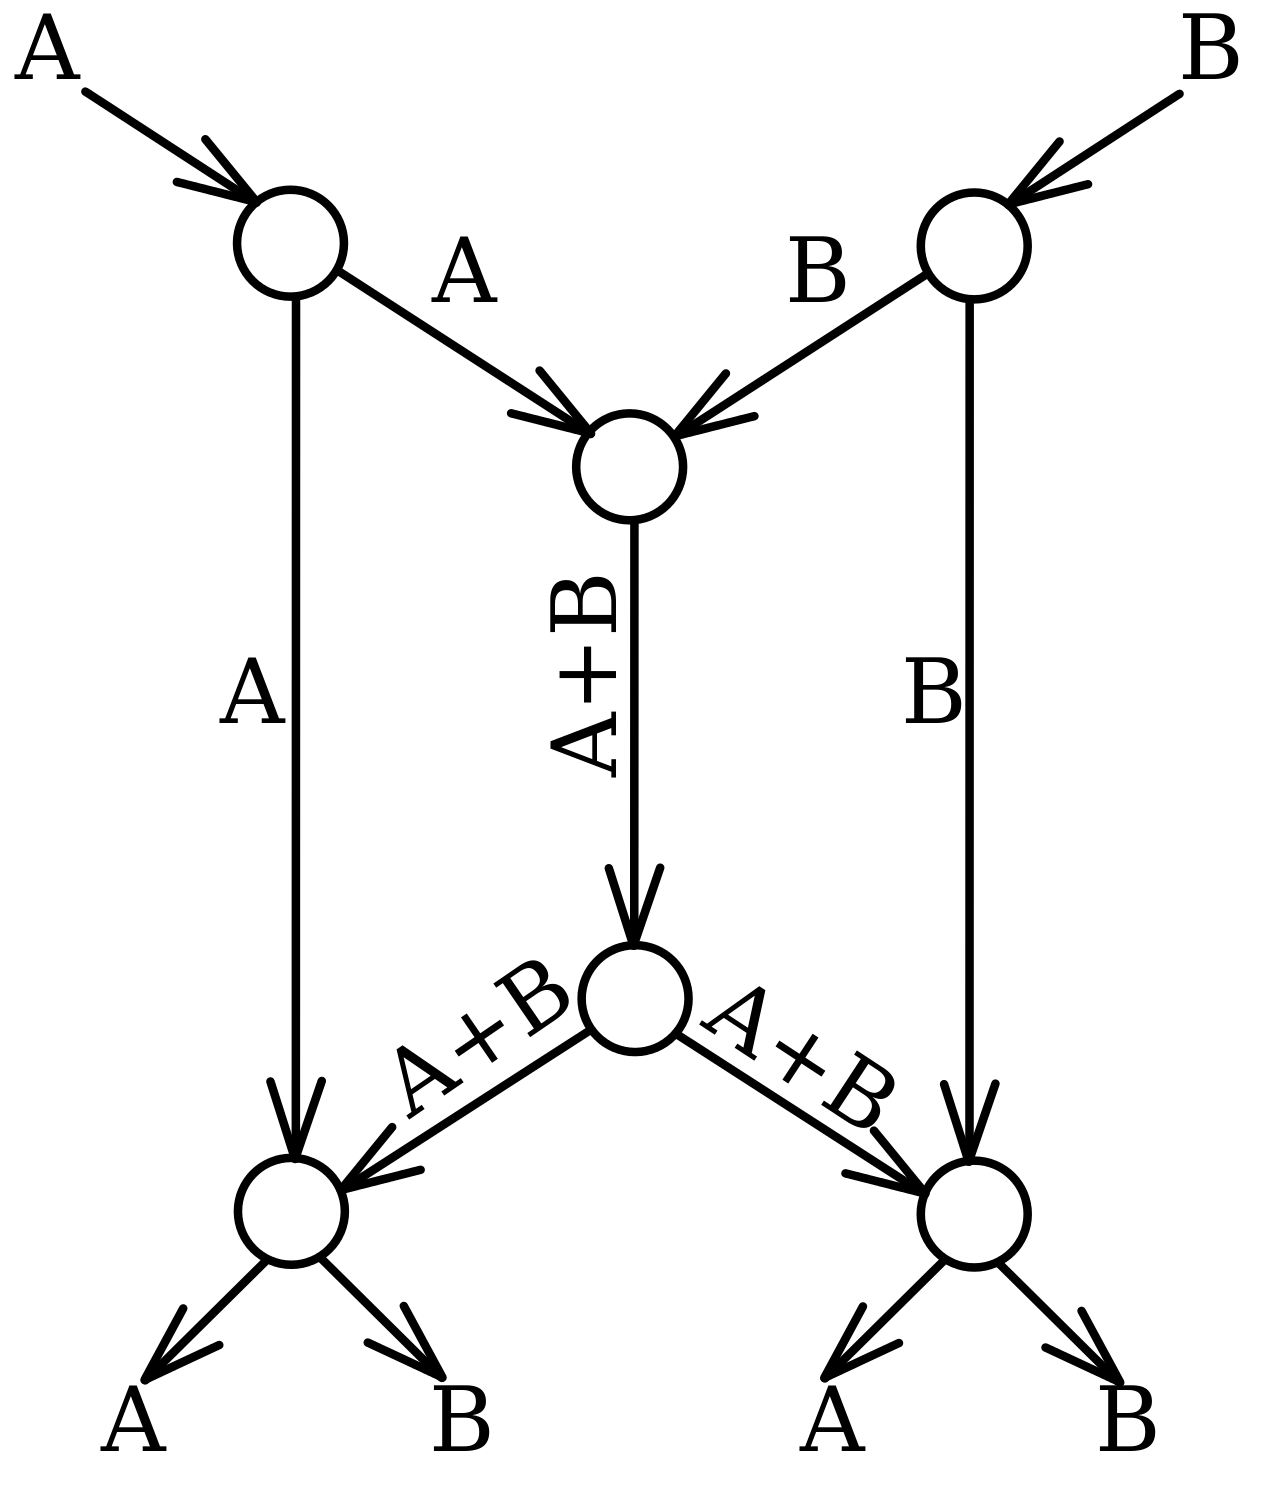
\includegraphics[scale=0.15]{images/Butterfly_network.svg.png}
                \caption{Exemple de Network Coding}
                \label{fig:exemple_Network_Coding}
            \end{figure}
            
            Comme on le voit ci-dessus, les paquets \textbf{A} et \textbf{B} sont combinés pour former un paquet \textbf{A}+\textbf{B}. Ce paquet \textbf{A}+\textbf{B} n'est déchiffrable dans ce cas ci, seulement si on dispose du paquet \textbf{A} ou du paquet \textbf{B}.
            On retrouvera par exemple le paquet \textbf{B} en faisant : (\textbf{A}+\textbf{B}) - \textbf{A} = \textbf{B}.
            \\
            
    \item [•] Absence de connectivité Internet :
    \\
    le système n'utilisera que les SMS
    \\
    
    \item [•] Equilibrage de la charge énergétique et de l'empreinte carbone :
    \\
    les différents slots de l'image passeront par différents mobiles intermédiaires
    de membres du réseau social
    \\
    
    \item [•]  Confidentialité :
    \\
     les numéros de mobiles des participants doivent rester confidentiels.
     Un serveur central sera donc utilisé pour gérer l'association
     pseudonyme-numéro
     \\
     \item [•] Environnement non sécurisé avec risques de perte de messages
        et d'injection de faux messages :
        \\
        une PKI sera mise en place pour assurer l'authentification des participants
     \\
     
     \item [•] Optimisation de la bande passante :
     \\
    la technique du Network Coding sera utilisée

\end{itemize}

\section{Architecture}

\section{Diagramme de Gantt}

    \begin{figure}[H]
        \centering
        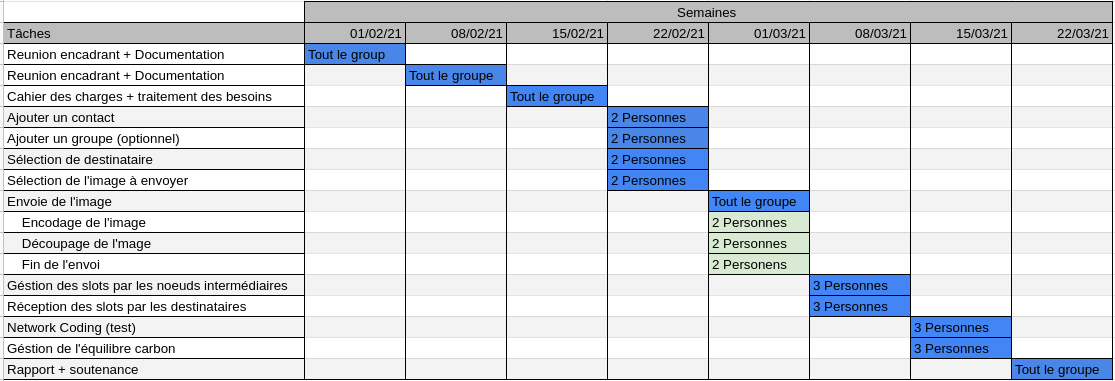
\includegraphics[scale=0.4]{images/gantt.png}
        \caption{Diagramme de Gantt}
        \label{fig:diagramme_gantt}
    \end{figure}

\section{Analyse du fonctionnement}

\section{Ressources allouées}
%Humain, financier, matériel, temporel

\section{Conclusion}

\end{document}
